\documentclass[a4paper, brazilian]{article}
\usepackage{config}

\usepackage{wasysym}
\usepackage{textcomp}

\begin{document}

\begin{titlepage}
		\begin{center}
			\begin{large}
				\textbf{Universidade Estadual de Campinas}\\\vspace{.5cm}
				\textbf{Faculdade de Engenharia Agrícola}\\\vspace{10.5cm}
			\end{large}
			\begin{large}
				\uppercase{\textbf{Cargas de contato e determinação do módulo de firmeza}}\\\vspace{4cm}
			\end{large}
		\end{center}
		\begin{large}
			\noindent\textbf{Nome:} \href{https://github.com/RenanSGuedes/576}{Renan da Silva Guedes}\\\\
			\noindent\textbf{RA:} 223979\\\vspace{5cm}
		\end{large}
		\begin{center}
			\begin{large}
				Campinas\\\vspace{.3cm}
				2020
			\end{large}
		\end{center}
	\end{titlepage}
	
	\newpage
	
	\section{Introdução}
	
	O ensaio realizado consiste na determinação do módulo de firmeza (\textit{firmness}) de diferentes materiais quando submetidos à compressão.
	Segundo NELSON, MOHSENIN (1968), o termo ``\textit{firmness}''
	pode ser usado para comparação do módulo de elasticidade de materiais biológicos. É descrito como uma característica elástica desses materiais, e definido por
	
	\begin{equation}
		\textit{firmness}=\dfrac{E}{1-\nu^{2}}
	\end{equation}
	sendo $E$ o módulo de elasticidade e $\nu$ o coeficiente de Poisson do material.
	
	\section{Objetivo}
	
	Determinação do Módulo Firmness
	
	\section{Materiais e métodos}
	
	Os materiais utilizados foram a laranja, esfera e cilindro de silicone, paquímetro digital, Máquina universal de Ensaios e \textit{software} para aquisição de dados.
	
	O procedimento realizado foi baseado no que é visto na \cref{fig:method},  sendo requerida sua execução para cada corpo de prova. No caso do cilindro, a aplicação da carga foi feita diametralmente, sendo  a velocidade da deformação dos corpos igual a \SI{1}{\milli\meter/\second}. Dessa forma, após aferir as medidas iniciais dos corpos e finalizar o ensaio foi obtido os valores presentes na \cref{tab:data}. Com o auxilio do \textit{software} para aquisição de dados chegou-se nos valores de carga máxima aplicada no ensaio de cada corpo (\cref{tab:load}).
	
	Em seguida, foi lançado mão das equações \eqref{lobo} e \eqref{hertz} para a obtenção do módulo de \textit{firmness}. A equação \eqref{lobo} foi utilizada com os parâmetros coletados da compressão diametral do cilindro de silicone, enquanto \eqref{hertz} para a laranja e esfera devido suas geometrias.

	\section{Resultados e discussão}
	
	Após substituir os dados nas duas equações mencionadas anteriormente, foram obtidos os valores presentes na \cref{tab:firmness}, onde nota-se grande proximidade entre o \textit{firmness} da esfera e do cilindro (\SI{3.02}{\mega\pascal} e \SI{3.03}{\mega\pascal}, respectivamente). No caso da laranja, nota-se um módulo aproximadamente 81.5\% menor quando comparado à média dos módulos dos dois primeiros, evidenciando a maior suscetibilidade mecânica da mesma. Isso pode ter ocorrido devido ao fato da laranja ter menor capacidade de deformar antes de romper em relação ao silicone presente na esfera e cilindro, por exemplo.
	
	\section{Conclusão}
	
	A partir dos ensaios realizados, chega-se que corpos de prova de mesmo material, possuem módulos de \textit{firmness} bem próximos, demonstrando a independência da geometria dos corpos nesse caso. Enquanto que materiais de  menor firmness -- laranja estudada -- são caracterizados pela capacidade de deformação para a mesma carga aplicada quando comparado aos dois outros corpos.
	
	\section{Anexos}
	
	\begin{figure}[H]
		\centering
		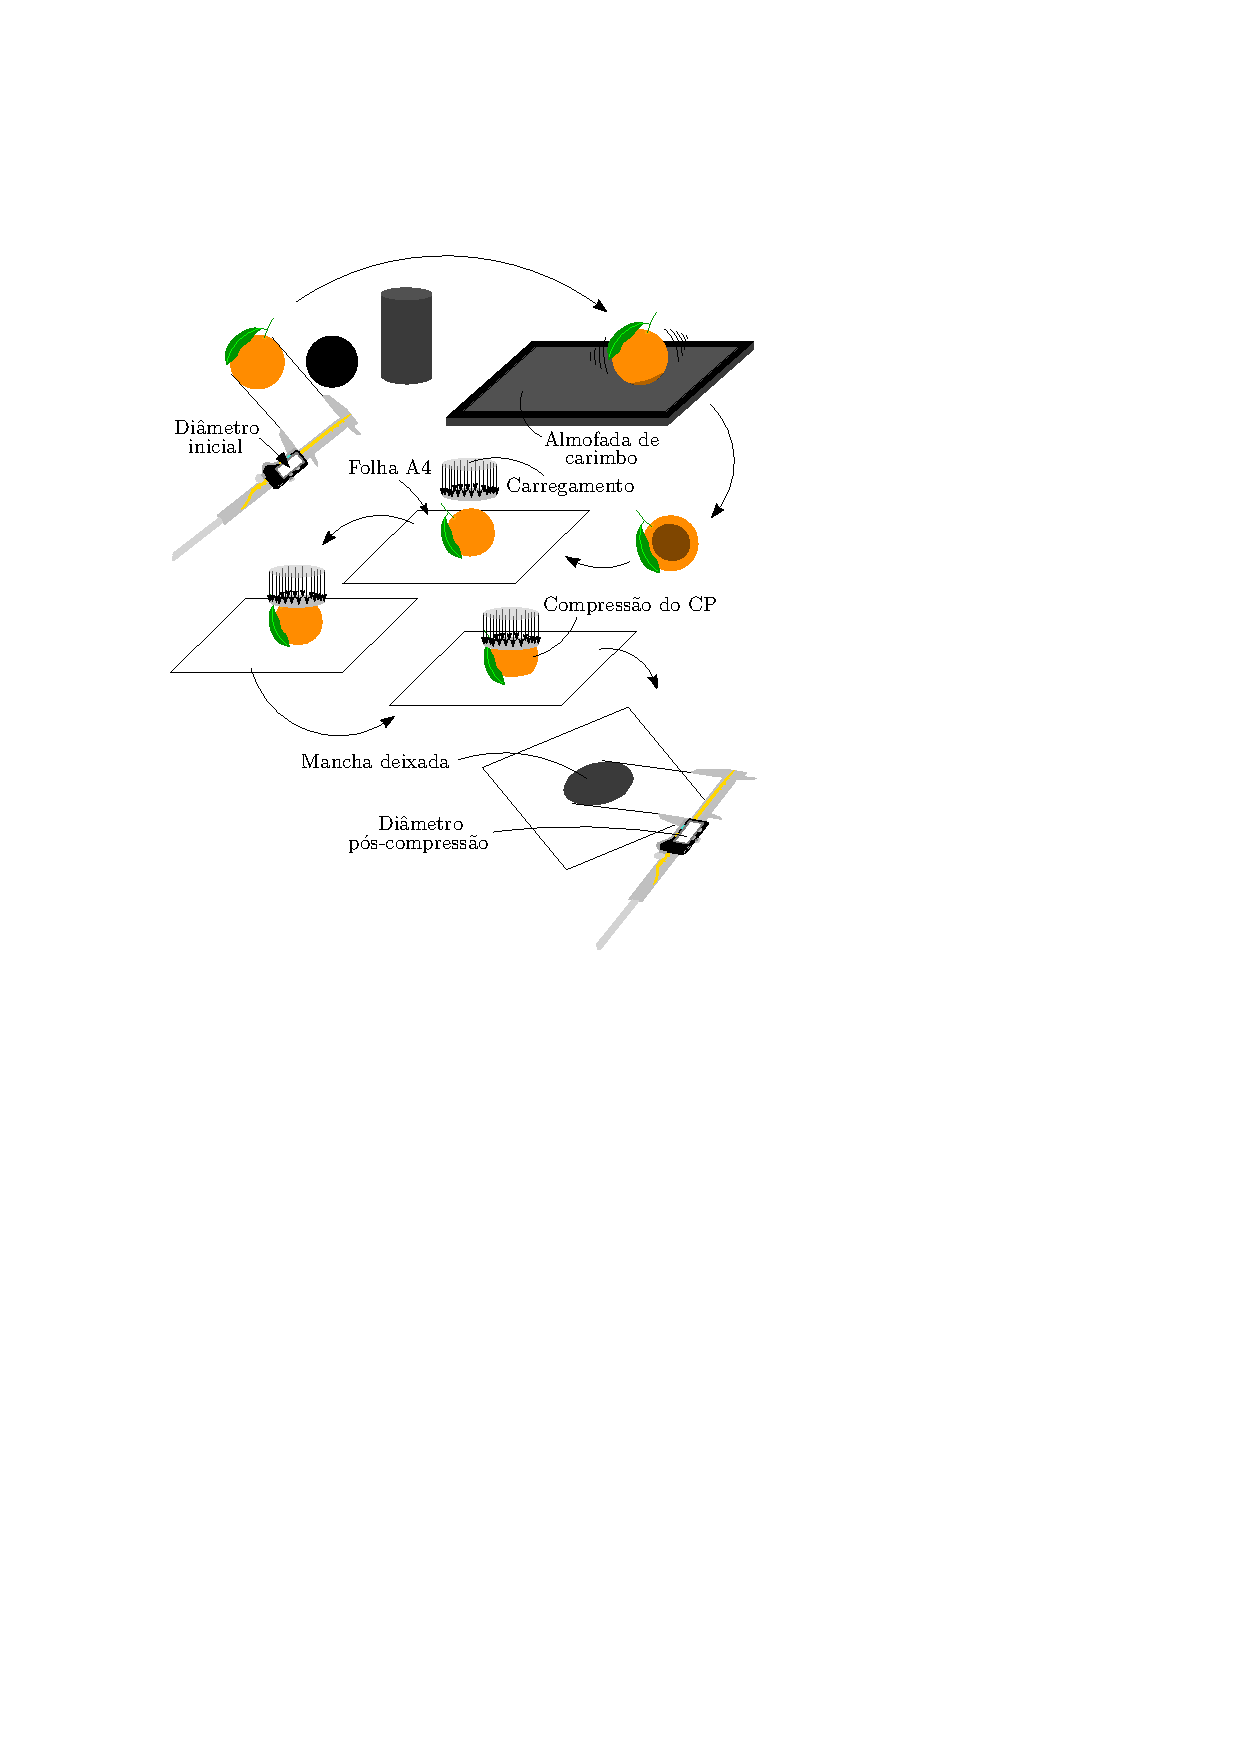
\includegraphics[scale=1]{images/xp3}
		\caption{Procedimentos adotados para os corpos de prova. O exemplo acima foi feita para a laranja como CP.}
		\label{fig:method}
	\end{figure}

	\subsection{Tabelas}
	
	\import{tables/}{data}
	
	\import{tables/}{firmness}

	\import{tables/}{load}
	
	\subsection{Equações}
		
	\begin{equation}
		\label{lobo}
		b=\sqrt{\dfrac{4\,F\,(1-\nu^{2})\,R}{\pi\,l\,E}}\Rightarrow \left(\dfrac{E}{1-\nu^{2}}\right)=\dfrac{4\,F\,R}{\pi\,l\,b^{2}}
	\end{equation}
	
	\begin{itemize}
		\item $b$ é a metade da largura da área de contato
		\item $l$ é o comprimento do cilindro (ou da área de contato)
		\item $R$ é o raio do corpo cilíndrico
		\item $F$ é a força aplicada (ortogonal ao plano de contato)
	\end{itemize}	
	
	\begin{equation}
		\label{hertz}
		a=\sqrt[3]{\dfrac{3\,F\,(1-\nu^{2})\,R}{4\,E}}\Rightarrow\left(\dfrac{E}{1-\nu^{2}}\right)=\dfrac{3\,F\,R}{4\,a^{3}}
	\end{equation}
	
	\begin{itemize}
		\item $a$ é o raio da área de contato
		\item $R$ é o raio do corpo esférico
		\item $F$ é a força aplicada (ortogonal ao plano de contato)
	\end{itemize}

	\section{Referências}
	
	MOHSENIN, N. N. \textbf{Physical properties of plant and animal materials}. 2.ed. New York: Gordon and Breach, 1986. 891p.
\end{document}